\documentclass[helvetica]{seminar} 
\input{xy}
\xyoption{all}
\usepackage{graphicx} 
\usepackage{slidesec} 
\usepackage{url}
\usepackage[usenames]{color}

\long\def\symbolfootnote[#1]#2{\begingroup%
\def\thefootnote{\fnsymbol{footnote}}\footnote[#1]{#2}\endgroup}

% to fix problems making landscape seminar pdfs
% Letter...
\pdfpagewidth=11truein
\pdfpageheight=8.5truein
\pdfhorigin=1truein     % default value(?), but doesn't work without
\pdfvorigin=1truein     % default value(?), but doesn't work without
% A4
%\pdfpagewidth=297truemm % your milage may vary....
%\pdfpageheight=210truemm
%\pdfhorigin=1truein     % default value(?), but doesn't work without
%\pdfvorigin=1truein     % default value(?), but doesn't work without



\renewcommand{\familydefault}{\sfdefault}  
 
\input{seminar.bug} 
\input{seminar.bg2} % See the Seminar bugs list 
 
\slideframe{none} 
 
 
\usepackage{fancyhdr} 
 
% Headers and footers personalization using the `fancyhdr' package 
\fancyhf{} % Clear all fields 
\renewcommand{\headrulewidth}{0mm} 
\renewcommand{\footrulewidth}{0.1mm} 
 
\fancyfoot[L]{\tiny RTCWEB Interim; Feb 2012} 
\fancyfoot[C]{\tiny Security}
\fancyfoot[R]{\tiny \theslide} 
 
 
% To center horizontally the headers and footers (see seminar.bug) 
\renewcommand{\headwidth}{\textwidth} 

% To adjust the frame length to the header and footer ones 
\autoslidemarginstrue 
\pagestyle{fancy} 
 

\newcommand{\heading}[1]{% 
  \begin{center} 
    \large\bf 
    #1 
  \end{center} 
  \vspace{.4 in}} 

\begin{document}
\begin{slide}
\begin{center}
\vspace{1 in}
\LARGE{{\bf}RTCWEB Architecture Open Issues}\\
\vspace{.2in}
\large{{Interim Meeting; February 2012}} \\
\vspace{3em}
\large{
\begin{tabular}{c}
Eric Rescorla \\
\url{ekr@rtfm.com}
\end{tabular}
}
\end{center}

\end{slide}


\centerslidesfalse

\begin{slide}
\heading{Overview}

\begin{itemize}
\item Security architecture document adopted after Taipei
  \begin{itemize}
  \item \verb^draft-ietf-rtcweb-security-arch-00^
  \end{itemize}
\item General agreement on a lot of issues
\item Purpose of the next 30 min
  \begin{itemize}
  \item Survey the open issues
  \item Resolve any that are easy
  \end{itemize}
\end{itemize}
\end{slide}


\begin{slide}
\heading{Issue: Mixed Content}

\begin{itemize}
\item Consent is granted by origin
\item What about active mixed content?
  \begin{itemize}
  \item \url{https://www.example.com/} loads script from \url{http://www.example.com}
  \item What are the PeerConnection permissions
  \end{itemize}

\item Current draft says: treat page as the HTTP origin
  \begin{itemize}
  \item Browser security experts: \textbf{``NOOOOO!!!!!!!!''}
  \end{itemize}

\end{itemize}
\end{slide}



\begin{slide}
\heading{How Browsers Handle Active Mixed Content Now}

\begin{center}
\begin{tabular}{l p{2.5in}}
Browser & Action \\
\hline
Chrome & Allow with warning -- (soon to be block) \\
Firefox & Big warning dialog \\
IE & Block \\
Safari & Accept \\
\end{tabular}
\end{center}

\end{slide}



\begin{slide}
\heading{Proposed Resolution}

\begin{itemize}
\item MUST treat HTTP and HTTPS origins as separate [uncontroversial]
\item SHOULD~\symbolfootnote[1]{Should this be a MUST?} either:
  \begin{itemize}
  \item Forbid all active mixed content [better, but out of scope]
  \item Remove RTCWEB permissions for origins with mixed content
  \end{itemize}

\item Comments?
\end{itemize}

\vspace{.5in}
\end{slide}



\begin{slide}
\heading{Issue: Consent Freshness/Keepalives}

\begin{itemize}
\item Problem: How to verify continuing consent?
  \begin{itemize}
  \item Need some sort of keepalive
  \item ICE keepalives are STUN Binding Indications (one-way)
  \end{itemize}

\item Proposal: use STUN Binding Requests instead
  \begin{itemize}
  \item MUST check no less often than every 30s
  \end{itemize}

\item Comments?
\end{itemize}

\end{slide}

\begin{slide}
\heading{Issue: Media Security Requirements}

[TODO: background]

\end{slide}


\begin{slide}
\heading{Communications Security: Implementation Requirements (Proposed)}

\begin{itemize}
\item MUST implement DTLS-SRTP (for media) and DTLS (for data) 
\item MAY implement RTP(?) and SDES(??) for backward compatibility purposes 
\item Security MUST be default state
  \begin{itemize}
  \item Implementations MUST offer DTLS and/or DTLS-SRTP for every channel
  \item MUST accept DTLS and/or DTLS-SRTP whenever offered 
  \item MUST not do unencrypted data channel
  \end{itemize}
\end{itemize}

\end{slide}



\centerslidestrue

\begin{slide}
\begin{center}
\vspace{1 in}
\LARGE{{\bf}RTCWEB Generic Identity Service}\\
\vspace{.2in}
\large{{Interim Meeting; February 2012}} \\
\vspace{3em}
\large{
\begin{tabular}{c}
Eric Rescorla \\
\url{ekr@rtfm.com}
\end{tabular}
}
\end{center}

\end{slide}


\centerslidesfalse



\begin{slide}
\heading{What are we trying to accomplish?}

\begin{itemize}
\item Allow Alice and Bob to have a secure call
  \begin{itemize}
  \item Authenticated with their identity providers
  \item On any site
    \begin{itemize}
    \item Even untrusted/partially trusted ones
    \end{itemize}
  \end{itemize}

\item Advantages
  \begin{itemize}
  \item Use one identity on any calling site
  \item Security against active attack by calling site
  \item Support for federated cases
  \end{itemize}
\end{itemize}

\end{slide}



\begin{slide}
\heading{Topology}

\begin{center}
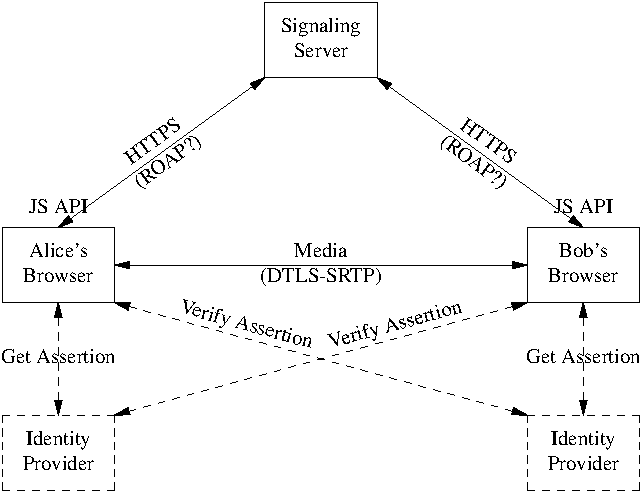
\includegraphics[width=3in]{full-topology}
\end{center}

\end{slide}



\begin{slide}
\heading{Terminology}
\begin{itemize}
\item[] \emph{Authenticating Party (AP)}:  The entity which is trying to establish its identity.

\item[] \emph{Identity Provider (IdP)}:  The entity which is vouching for the AP's identity.

\item[] \emph{ Relying Party (RP)}:  The entity which is trying to verify the AP's identity.
\end{itemize}

\end{slide}





\begin{slide}
\heading{Types of IdP}

\begin{itemize}
\item[] \emph{Authoritative}: Attests for identities within their own namespace
  \begin{itemize}
  \item Often multiple Authoritatives IdPs exist with different scopes
  \item Examples: DNSSEC, RFC 4474, Facebook Connect (for the Facebook ID)
  \end{itemize}

\item[] \emph{Third-party}: Attests for identities in a name-space they don't control
  \begin{itemize}
  \item Often multiple Third-Party IdPs share the same space
  \item Can attest to real-world identities
  \item Examples: SSL/TLS certificates, the State of California (driver's licenses)
  \end{itemize}
\end{itemize}
\end{slide}


\begin{slide}
\heading{Authoritative vs. Third-Party IdPs: Trust Relationship}

\begin{itemize}
\item No need to explicitly trust third-party IdPs
  \begin{itemize}
  \item \url{ekr@example.com} is whoever \url{example.com} says it is
  \item The problem is authenticating \url{example.com}
  \end{itemize}

\item Authoritative IdPs need to be explicitly trusted
  \begin{itemize}
  \item Example: how do I know GoDaddy is a legitimate CA?
  \item Answer: the browser manufacturer vetted them
  \item They are allowed to attest to \emph{any} domain name
  \end{itemize}
\end{itemize}
\end{slide}


\begin{slide}
\heading{User Relationships with IdPs}

\begin{itemize}
\item Authenticating Party
  \begin{itemize}
  \item Has some account with the IdP
  \item May have established their identity 
    \begin{itemize}
    \item Especially for third-party IdPs
    \end{itemize}
  \item Can authenticate to the IdP in the future (e.g., with a password)
  \end{itemize}

\item Relying party
  \begin{itemize}
  \item Doesn't have any account relationship with the IdP\symbolfootnote[1]{Note: privacy issues.}
  \item Must be able to verify the IdP's identity
  \item Needs to trust third-party IdPs
  \end{itemize}

\end{itemize}
\end{slide}


\begin{slide}
\heading{Web-based IdP Systems}

\begin{itemize}
\item Facebook Connect
\item Google login
\item OAuth
\item OpenID
\item BrowserID
\end{itemize}

\end{slide}



\begin{slide}
\heading{Example: Facebook Connect (sorta OAuth)}

\begin{itemize}
\item AP is a user with a Facebook account
  \begin{itemize}
  \item They may or may not be logged in at the moment
  \item (Where \emph{logged in} == cookies)
  \end{itemize}

\item RP is a Web server
  \begin{itemize}
  \item Idea is to bootstrap Facebook authentication
  \item ... rather than have your own account system
  \item RP registers with Facebook and gets an application key
  \end{itemize}
\end{itemize}
\end{slide}



\begin{slide}
\heading{Facebook Connect Call Flow (not logged in) 1}

\vspace{-.7in}
$$
\xymatrix@C=1.0in@R=.15in{
  \txt{Alice} & \txt{RP\\\url{www.example.com}} & \txt{Facebook} \\
  \ar[r]^{\txt{\texttt{GET /...}}} & & \\
  & \ar[l]_{\txt{Redirect to}}^{\txt\tiny{\texttt{www.facebook.com/dialog/oauth?client\_id=1234\&redirect\_uri=www.example.com/auth}}} & \\
  \ar[rr]^{\txt\tiny{\texttt{GET /dialog/oauth?client\_id=1234\&redirect\_uri=www.example.com/auth}}} & & \\
  & & \ar@{<->}[ll]_{\txt{Login and permissions dialog}} \\
}
$$

\end{slide}



\begin{slide}

\begin{center}
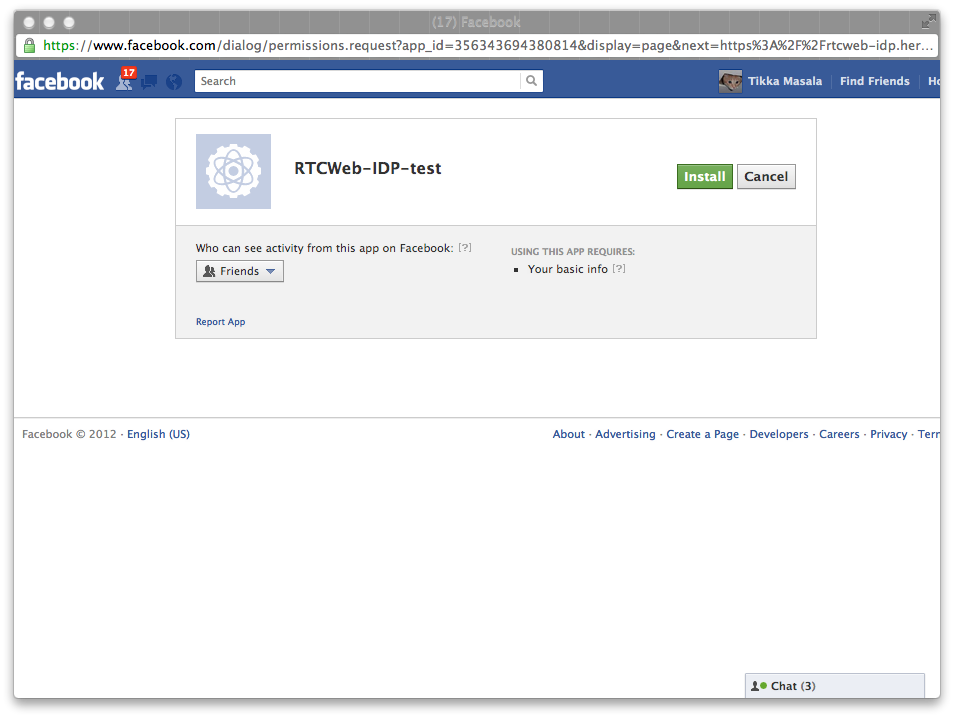
\includegraphics[width=3.5in]{fb-permissions}
\end{center}

\end{slide}

\begin{slide}
\heading{Facebook Connect Call Flow (not logged in) 2}

\vspace{-.7in}
$$
\xymatrix@C=1.0in@R=.15in{
  \txt{Alice} & \txt{RP\\\url{www.example.com}} & \txt{Facebook} \\
  \ar[r]^{\txt{\texttt{GET /...}}} & & \\
  & \ar[l]_{\txt{Redirect to}}^{\txt\tiny{\texttt{www.facebook.com/dialog/oauth?client\_id=1234\&redirect\_uri=www.example.com/auth}}} & \\
  \ar[rr]^{\txt\tiny{\texttt{GET /dialog/oauth?client\_id=1234\&redirect\_uri=www.example.com/auth}}} & & \\
  & & \ar@{<->}[ll]_{\txt{Login and permissions dialog}} \\
  & & \ar[ll]_{\txt{Redirect to}}^{\txt\tiny{\texttt{www.example.com/auth?code=5678}}}\\
  \ar[r]^{\txt\tiny{\texttt{GET /auth?code=5678}}} & &\\
  & \ar[r]^{\txt\tiny{\texttt{GET /oauth/access\_token?client\_id=1234\&client\_secret=<secret>\&code=5678}}} & \\
  & & \ar[l]_{\txt\tiny{\texttt{access\_token=987654321}}} \\
  & \ar[r]^{\txt\tiny{\texttt{GET /me?access\_token=987654321}}} & \\
  & & \ar[l]_{\txt\tiny{\texttt{user=1111111, ...}}} \\
  & \ar[l]_{\txt{Hello, user 1111111}} & \\
}
$$

\end{slide}




\begin{slide}
\heading{Facebook Connect Call Flow (logged in)}

\vspace{-.7in}
$$
\xymatrix@C=1.0in@R=.15in{
  \txt{Alice} & \txt{RP\\\url{www.example.com}} & \txt{Facebook} \\
  \ar[r]^{\txt{\texttt{GET /...}}} & & \\
  & \ar[l]_{\txt{Redirect to}}^{\txt\tiny{\texttt{www.facebook.com/dialog/oauth?client\_id=1234\&redirect\_uri=www.example.com/auth}}} & \\
  \ar[rr]^{\txt\tiny{\texttt{GET /dialog/oauth?client\_id=1234\&redirect\_uri=www.example.com/auth}}} & & \\
  & & \ar[ll]_{\txt{Redirect to}}^{\txt\tiny{\texttt{www.example.com/auth?code=5678}}}\\
  \ar[r]^{\txt\tiny{\texttt{GET /auth?code=5678}}} & &\\
  & \ar[r]^{\txt\tiny{\texttt{GET /oauth/access\_token?client\_id=1234\&client\_secret=<secret>\&code=5678}}} & \\
  & & \ar[l]_{\txt\tiny{\texttt{access\_token=987654321}}} \\
  & \ar[r]^{\txt\tiny{\texttt{GET /me?access\_token=987654321}}} & \\
  & & \ar[l]_{\txt\tiny{\texttt{user=1111111, ...}}} \\
  & \ar[l]_{\txt{Hello, user 1111111}} & \\
}
$$

\end{slide}


\begin{slide}
\heading{Facebook Connect Privacy Features}

\begin{itemize}
\item RP needs to register with Facebook
\item User approves policy separately for each RP
  \begin{itemize}
  \item Including which user information to share
  \end{itemize}

\item Facebook learns about every authentication transaction
  \begin{itemize}
  \item Including user/RP pair
  \end{itemize}

\end{itemize}

\end{slide}


\begin{slide}
\heading{Example: BrowserID (no key pair)}

\vspace{-.5in}
$$
\xymatrix@C=0.8in@R=.15in{
  \txt{Alice} & \txt{RP\\\url{www.example.com}} & \txt{BrowserID.org} \\
    \ar[r]^{\txt{\texttt{GET /...}}} & & \\
    & \ar[l]_{\txt\tiny{\texttt{<script src="https://browserid.org/include.js"/>}}}^{\txt\tiny{\texttt{navigator.id.get(function(assertion)\{...\});}}} & \\
    \txt{[Generate Keys]} \\
    \ar[rr]^{\txt{Get certificate + Cookie}} & & \\
    & & \ar[ll]_{\txt{Certificate}} \\
    \txt{[Sign Assertion]} \\
    \ar[r]^{\txt{Signed assertion + Certificate}} & \\
    & \ar[l]_{\txt{Hello, user 11111111}} \\
}
$$

\end{slide}

\begin{slide}

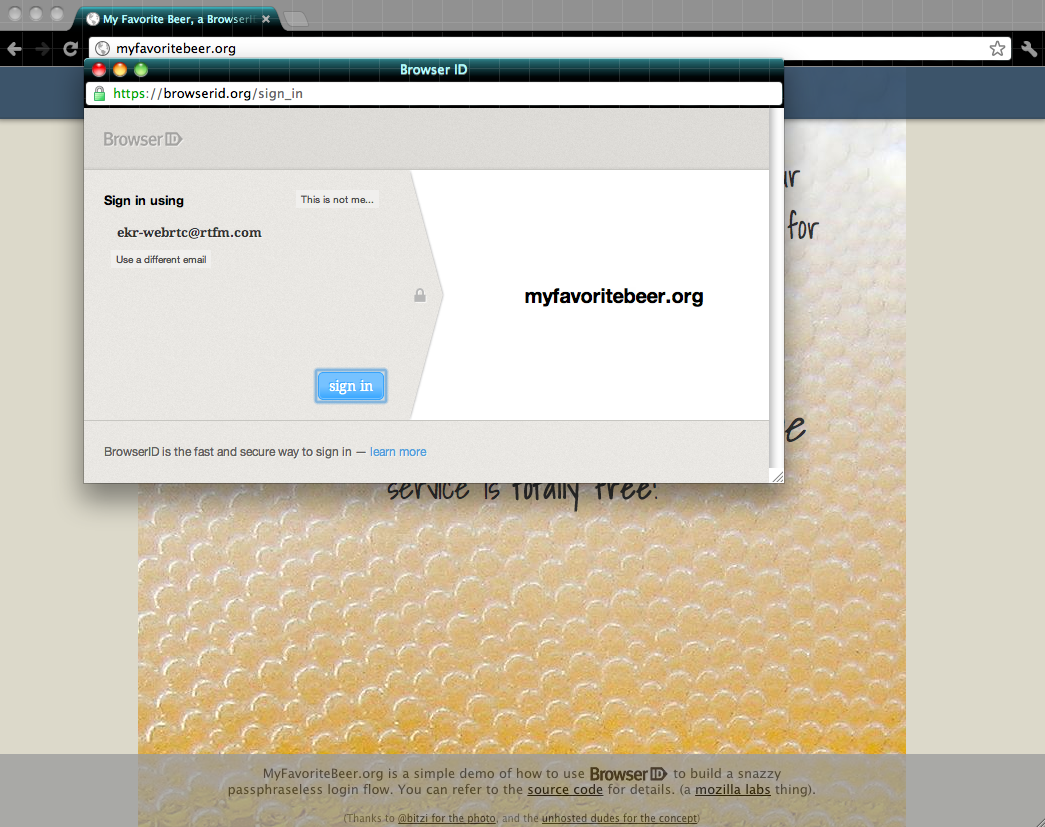
\includegraphics[width=4in]{browserid-login.png}

\end{slide}





\begin{slide}
\heading{BrowserID: Why no MITM Attacks?}

\vspace{-.5in}
$$
\xymatrix@C=0.7in@R=.15in{
  \txt{Alice} & \txt{\url{attacker.com}} & \txt{\url{example.com}} \\
    \ar[r]^{\txt{\texttt{GET /...}}} & & \\
    & \ar[r]^{\txt{\texttt{GET /...}}} & \\
    & \ar[l]_{\txt\tiny{\texttt{<script src="https://browserid.org/include.js"/>}}}^{\txt\tiny{\texttt{navigator.id.get(function(assertion)\{...\});}}} & \\
    \txt{[Sign Assertion]} \\
    \ar[r]^{\txt{Signed assertion + Certificate}} & \\
    &   \ar[r]^{\txt{Signed assertion + Certificate}} & \\
    & & \ar[l]_{\txt{Hello, user 11111111}} \\
}
$$
\end{slide}

\begin{slide}
\heading{BrowserID: Audience Parameter}

\vspace{-.5in}
$$
\xymatrix@C=0.7in@R=.15in{
  \txt{Alice} & \txt{\url{attacker.com}} & \txt{\url{example.com}} \\
    \ar[r]^{\txt{\texttt{GET /...}}} & & \\
    & \ar[r]^{\txt{\texttt{GET /...}}} & \\
    & \ar[l]_{\txt\tiny{\texttt{<script src="https://browserid.org/include.js"/>}}}^{\txt\tiny{\texttt{navigator.id.get(function(assertion)\{...\});}}} & \\
    \txt{[Sign Assertion]} \\
    \ar[r]^{\txt{Signed assertion({\color{blue} audience=\texttt{attacker.com}}) + Certificate}} & \\
    &   \ar[r]^{\txt{Signed assertion + Certificate}} & \\
    & & \ar[l]_{\txt{Audience mismatch error}} \\
}
$$
\end{slide}

\begin{slide}
\heading{Preventing assertion forwarding}

\begin{itemize}
\item BrowserID assertions are scoped to origin (audience parameter)
  \begin{itemize}
  \item RPs check that the origin in the assertion matches their domain
  \item This prevents assertion forwarding
  \end{itemize}

\item Why does this work?
  \begin{itemize}
  \item BrowserID JS is part of the TCB
  \item Browser enforces origin of requests from the calling site
  \item RP transitively trusts origin/audience because it trusts BrowserID.org
  \end{itemize}
\end{itemize}

\end{slide}
        



\begin{slide}
\heading{Browser-ID Privacy Features}

\begin{itemize}
\item Client generates a key pair
  \begin{itemize}
  \item Idp signs a binding between key pair and user ID
  \end{itemize}

\item Client generates assertions based on key pair
  \begin{itemize}
  \item Sends along certificate
  \end{itemize}

\item RP fetches IdP public key
  \begin{itemize}
  \item This need only happen once
  \end{itemize}

\item IdP never learns where you are visiting
  \begin{itemize}
  \item No relationship between RP and IdP
  \end{itemize}


\end{itemize}

\end{slide}


\begin{slide}
\heading{Example: BrowserID (existing key pair)}

\vspace{-.5in}
$$
\xymatrix@C=0.8in@R=.15in{
  \txt{Alice} & \txt{RP\\\url{www.example.com}} & \txt{BrowserID.org} \\
    \ar[r]^{\txt{\texttt{GET /...}}} & & \\
    & \ar[l]_{\txt\tiny{\texttt{<script src="https://browserid.org/include.js"/>}}}^{\txt\tiny{\texttt{navigator.id.get(function(assertion)\{...\});}}} & \\
    \txt{[Sign Assertion]} \\
    \ar[r]^{\txt{Signed assertion + Certificate}} & \\
    & \ar[l]_{\txt{Hello, user 11111111}} \\
}
$$

\end{slide}





\begin{slide}
\heading{BrowserID Security Architecture}

\begin{center}
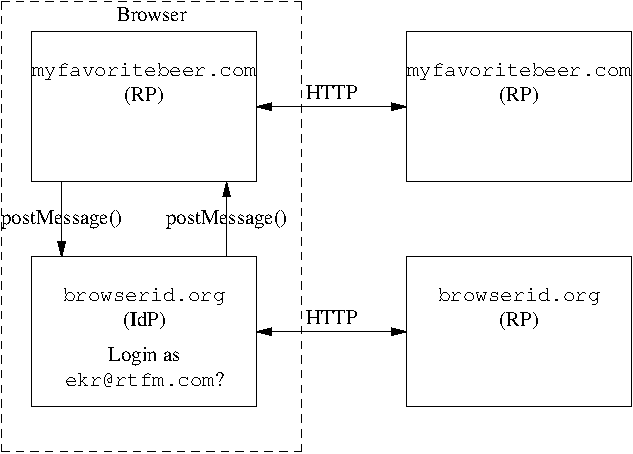
\includegraphics[width=3.2in]{browserid-arch}
\end{center}

\end{slide}


\begin{slide}
\heading{One browser, multiple security contexts}

\begin{itemize}
\item Browser security data scoped by \emph{origin}
  \begin{itemize}
  \item \url{browserid.org} window and \url{myfavoritebeer.org} window are isolated
  \item Each runs their own JS independently
  \end{itemize}

\item Security guarantees
  \begin{itemize}
  \item Origin A can't touch origin B's data
  \item Origin A can't see what origin B is displaying
  \item Communication is by \verb^postMessage()^ (or navigation hack)
  \end{itemize}
\end{itemize}
\end{slide}


\begin{slide}
\heading{PostMessage: Sender}

\verb^otherWindow.postMessage(message, targetOrigin);^

\begin{itemize}
\item[] \verb^otherWindow^: the window to send the message to
\item[] \verb^message^: the message to send
\item[] \verb^targetOrigin^: the expected origin of the other window
\end{itemize}
\end{slide}


\begin{slide}
\heading{Why do we need \texttt{targetOrigin}?}

\begin{itemize}
\item Malicious pages can navigate other windows
  \begin{itemize}
  \item This creates a race condition
  \end{itemize}

\item RP creates the new window to IdP with \verb^w = createWindow()^
\item Attacker navigates \verb^w^ to his own site
\item RP does \verb^w.postMessage(secret,...)^
\item Attacker gets the secret
\item \verb^targetOrigin^ stops this
\end{itemize}

\end{slide}


\begin{slide}
\heading{PostMessage: receiver}

\begin{verbatim}
window.addEventListener('message',
                        function(event) {
                          ...
                        });
\end{verbatim}

\begin{itemize}
\item Event properties:
  \begin{itemize}
  \item[] \verb^data^: the message passed by the sender
  \item[] \verb^origin^: the sender's origin
  \item[] \verb^source^: the sender's window
  \end{itemize}

\item Important: \verb^origin^ value can be trusted
  \begin{itemize}
  \item Enforced by the browser
  \item May not be the current origin of \verb^source^, however
  \end{itemize}
\end{itemize}
\end{slide}


\begin{slide}
\heading{IFRAMEs}

\begin{itemize}
\item What if I don't want another window to open?
  \begin{itemize}
  \item Solution: IFRAMEs
  \end{itemize}

\end{itemize}

\end{slide}


\end{document}